\documentclass[journal]{IEEEtran}

\usepackage{cite}
\usepackage{amsmath,amssymb,amsfonts}
\usepackage{algorithmic}
\usepackage{graphicx}
\usepackage{textcomp}
\usepackage{xcolor}
\usepackage{booktabs}
\usepackage{multirow}
\usepackage{array}
\usepackage{url}
\usepackage{hyperref}
\usepackage{pgfplots}
\usepackage{pgfplotstable}
\usepackage{tikz}
\usetikzlibrary{shapes.geometric, arrows, positioning}
\pgfplotsset{compat=1.18}

\hypersetup{
    colorlinks=true,
    linkcolor=blue,
    citecolor=blue,
    urlcolor=blue
}

\begin{document}

\title{Graph-Based and Self-Supervised Knowledge Tracing in Sparse-Concept Settings: A Systematic Survey and Research Agenda}

\author{Khanh-Trinh~Nguyen, Tuan~Dao~Minh, Duong~Nguyen~Tien, Chi~Thanh~Nguyen, and~Van-Hau~Nguyen*%
\thanks{Khanh-Trinh Nguyen, Tuan Dao Minh, Duong Nguyen Tien, and Van-Hau Nguyen are with the Faculty of Information Technology, Hung Yen University of Technology and Education, Hung Yen 160000, Vietnam (e-mail: trinhnk@utehy.edu.vn; tuandm@utehy.edu.vn; duongnt@utehy.edu.vn; haunv@utehy.edu.vn).}%
\thanks{Chi Thanh Nguyen is with the Academy of Military Science and Technology, Ha Noi 100000, Vietnam (e-mail: thanhnc@amst.edu.vn).}%
\thanks{*Corresponding author: Van-Hau Nguyen (e-mail: haunv@utehy.edu.vn).}}

\markboth{IEEE Transactions on Learning Technologies,~2026}%
{Nguyen \MakeLowercase{\textit{et al.}}: Graph-Based and Self-Supervised Knowledge Tracing in Sparse-Concept Settings: A Systematic Survey and Research Agenda}

\IEEEtitleabstractindextext{%
\begin{abstract}
Knowledge Tracing (KT) is a foundational task in Educational Data Mining (EDM) and Intelligent Tutoring Systems (ITS), sequentially predicting student mastery over Knowledge Components (KCs) from interaction logs. Traditional deep KT models treat exercise and concept identifiers as categorical tokens, ignoring explicit domain structures and suffering representation collapse under interaction data sparsity. To address these bottlenecks, Graph-Based KT (Graph-KT) and Self-Supervised KT (SSL-KT) paradigms have rapidly emerged. However, literature lacks a systematic synthesis evaluating how graph topologies, self-supervised pretext tasks, and sparse evaluation protocols interact. Following the PRISMA 2020 statement, this paper presents a comprehensive systematic review of 37 primary core studies (2018--2026) selected across seven electronic databases ($N = 2,017$ initial records). We establish a two-dimensional taxonomy classifying Graph-KT along graph provenance (expert, log-based, dynamic, LLM AST) and GNN encoder axes (GCN, GAT, heterogeneous, hypergraph, dynamic), and SSL-KT across four pretext task families (multi-view contrastive, graph structural, hypergraph contrastive, generative masked auto-encoding). Methodologically, we expose a critical vulnerability: 94.6\% of studies claim to address data sparsity, yet only 5.4\% evaluate under strict zero-exposure concept cold-start. Standard models collapse near random guessing under zero-exposure splits because GNN message passing over co-occurrence graphs lacks inductive out-of-vocabulary mechanisms. Furthermore, 0 out of 37 studies report probability calibration (ECE), posing risks for adaptive tutoring decisions. We formulate six evidence-derived research agenda pillars with formal mathematical specifications, laying the foundation for trustworthy learning technologies.
\end{abstract}

\begin{IEEEkeywords}
Knowledge Tracing, Graph Neural Networks, Self-Supervised Learning, Sparse Concepts, Cold-Start Learning, Systematic Literature Review, Educational Data Mining, Intelligent Tutoring Systems.
\end{IEEEkeywords}}

\maketitle
\IEEEdisplaynontitleabstractindextext
\IEEEpeerreviewmaketitle

% ─────────────────────────────────────────────────────────────────────────────
% SECTION 1: INTRODUCTION
% ─────────────────────────────────────────────────────────────────────────────
\section{Introduction}
\label{sec:intro}

\IEEEPARstart{K}{nowledge} Tracing (KT) is the fundamental task of sequentially modeling student mastery over educational Knowledge Components (KCs, e.g., concepts, skills, rules) based on historical learning interaction logs. In modern Intelligent Tutoring Systems (ITS), Educational Data Mining (EDM), and adaptive learning environments, Knowledge Tracing serves as the algorithmic engine for personalized learning pathways, learner-state estimation, step-based scaffolding, and automated curriculum adaptation. Formally, given a sequence of $T$ student interaction tuples $\mathcal{X}_{1:T} = \{(x_1, r_1), (x_2, r_2), \dots, (x_T, r_T)\}$, where $x_t \in \mathcal{E}$ represents the exercise or concept attempted at time $t$, and $r_t \in \{0, 1\}$ indicates the binary response accuracy (0 for incorrect, 1 for correct), the goal of Knowledge Tracing is to predict the response probability $P(r_{T+1} = 1 \mid x_{T+1}, \mathcal{X}_{1:T})$ on a target exercise $x_{T+1}$. Table~\ref{tab:notation_summary} summarizes the principal mathematical notations used throughout this survey.

\begin{table*}[t]
\caption{Summary of Key Mathematical Notations}
\label{tab:notation_summary}
\centering
\resizebox{0.92\textwidth}{!}{
\begin{tabular}{@{}lp{10cm}@{}}
\toprule
\textbf{Symbol} & \textbf{Mathematical Definition / Meaning} \\
\midrule
$\mathcal{X}_{1:T}$ & Sequential interaction history of a student up to time $T$ \\
$x_t, r_t$ & Exercise/concept attempted at time $t$ and binary response $r_t \in \{0,1\}$ \\
$\mathcal{E}, \mathcal{K}$ & Repository sets of exercises and Knowledge Components (KCs) \\
$\mathbf{A} \in \mathbb{R}^{|\mathcal{K}| \times |\mathcal{K}|}$ & Concept graph adjacency matrix (co-occurrence / prerequisite) \\
$h_k^t \in \mathbb{R}^d$ & Dynamic hidden knowledge state representation of concept $k$ \\
$\mathbf{Z}^{(v)}$ & Node/view representation embedding matrix from GNN view $v$ \\
$\tau$ & Temperature hyperparameter in InfoNCE contrastive loss \\
$\mathbb{B}^d$ & $d$-dimensional Poincaré hyperbolic ball manifold \\
$\oplus_{\mathbf{c}}$ & Möbius addition operator under curvature parameter $\mathbf{c}$ \\
$\text{ECE}$ & Expected Calibration Error metric for probability calibration \\
\bottomrule
\end{tabular}
}
\end{table*}

Since the seminal Deep Knowledge Tracing (DKT) model \cite{Piech_DKT_2015} introduced Recurrent Neural Networks (RNNs) to sequence modeling in education, deep learning models---including Attention-based KT (SAKT \cite{Pandey_SAKT_2019}, AKT \cite{Ghosh_AKT_2020}) and Memory Network KT (DKVMN)---have dramatically improved predictive accuracy over classic psychometric baselines such as Bayesian Knowledge Tracing (BKT) and Item Response Theory (IRT).

\subsection{Learning-Technology Motivation: Data Sparsity \& Cold-Start}
Despite recent empirical progress, traditional deep KT architectures treat exercise and concept identifiers as independent categorical tokens, ignoring explicit domain structures and educational relationships. This formulation faces two severe bottleneck challenges in real-world intelligent tutoring systems:
\begin{enumerate}
    \item \textbf{Representation Collapse under Interaction Data Sparsity}: In realistic educational platforms, interaction matrices are extremely sparse. Most students attempt only a tiny fraction of the overall item repository, and long-tail concepts receive minimal interaction logs. Standalone sequence models fail to learn meaningful latent embeddings for sparse concepts, leading to severe representation collapse during learner-state estimation.
    \item \textbf{Strict Concept Cold-Start}: When new concepts or exercises are introduced into a curriculum without prior historical interaction logs, conventional deep KT models cannot infer student mastery. Handling zero-exposure concepts during curriculum adaptation requires incorporating external structural, pedagogical, or semantic knowledge graph priors.
\end{enumerate}

\subsection{Scope \& Gateway Criteria}
To address these fundamental limitations, two primary methodological paradigms have rapidly expanded:
\begin{itemize}
    \item \textbf{Graph-Based Knowledge Tracing (Graph-KT)}: Incorporating explicit graph or graph-structured relations (e.g., concept prerequisite trees, question-KC bipartite maps, dynamic co-occurrence graphs, relational paths, or hyperbolic skill manifolds) as a central structural mechanism, including but not limited to Graph Neural Network (GNN) message passing.
    \item \textbf{Self-Supervised Knowledge Tracing (SSL-KT)}: Formulating auxiliary pre-training or contrastive pretext tasks (e.g., multi-view graph contrast, masked auto-encoding) to regularize student state representations.
\end{itemize}

Our systematic survey enforces a strict, frozen primary-corpus gateway rule:
\begin{equation}
\begin{split}
\text{PRIMARY\_CORE} = \; & \text{KT} \land (\text{GRAPH\_BASED} \\
& \lor \text{SELF\_SUPERVISED})
\end{split}
\end{equation}

Only studies where Knowledge Tracing is the central prediction task AND that leverage explicit Graph-Based or Self-Supervised mechanisms are included in our primary synthesis corpus.

\subsection{Comparison with Prior Reviews and Benchmarks}
While previous reviews and benchmark suites have examined deep learning in education generally (e.g., Abdelrahman et al. \cite{Abdelrahman_Survey_2023}), benchmarked sequence models (e.g., pyKT \cite{Liu_pyKT_2022}), or reviewed standard GNN applications in EDM (e.g., Wang et al. \cite{Wang_GraphKT_2024}), our work provides a dedicated, PRISMA 2020-compliant systematic survey focusing specifically on Graph-Based and Self-Supervised KT paradigms under sparse-concept settings. Table~\ref{tab:survey_comparison} highlights key methodological differences across seven core survey dimensions.

\begin{table*}[t]
\caption{Comparison with Prior Knowledge Tracing Reviews and Benchmark Suites}
\label{tab:survey_comparison}
\centering
\resizebox{0.98\textwidth}{!}{
\begin{tabular}{@{}lcccc@{}}
\toprule
\textbf{Survey Dimension} & \textbf{Broad KT Surveys} \cite{Abdelrahman_Survey_2023} & \textbf{Deep-KT Benchmarks} \cite{Liu_pyKT_2022} & \textbf{Graph-KT Reviews} \cite{Wang_GraphKT_2024} & \textbf{This Survey (Ours, 2026)} \\
\midrule
Systematic Review Protocol & Narrative / Semi-systematic & Empirical Benchmark Code & Literature Review & \textbf{Full PRISMA 2020 (7 DBs, $N=2,017$)} \\
Graph Coverage \& Taxonomy & High-Level GNN Overview & Excluded (Sequence Baselines) & GNN-Focused Focus & \textbf{4-Family Provenance \& 5-Family GNN} \\
SSL Pretext Coverage & Minimal / None & Excluded & Minimal & \textbf{4-Family SSL Taxonomy ($N_S=14$)} \\
Sparse / Cold-Start Ontology & Generic Data Sparsity & Standard Interaction Splits & Interaction Sparsity & \textbf{Interaction Sparsity vs Zero-Exposure} \\
Graph Provenance Leakage & Not Audited & Not Audited & Not Audited & \textbf{Full Data Leakage \& Time Split Audit} \\
Probability Calibration (ECE) & Not Evaluated & AUC / ACC Only & Not Evaluated & \textbf{ECE Calibration Audit (0/37 Reported)} \\
Reproducibility \& Open Science & Citation Indexing & Code Repository & Paper Taxonomy & \textbf{Field-Level Evidence \& Open Science Audit} \\
\bottomrule
\end{tabular}
}
\end{table*}

\subsection{Main Contributions}
The main contributions of this systematic review are fourfold:
\begin{enumerate}
    \item \textbf{Comprehensive PRISMA 2020 Synthesis}: We execute a 7-database systematic search yielding 2,017 initial records, producing a verified primary core corpus of 37 Graph/SSL-KT studies ($N_G=31, N_S=14, N_{G \cap S}=8$).
    \item \textbf{Two-Dimensional Taxonomy Framework}: We establish a unified taxonomy classifying Graph-KT along Graph Provenance (Expert, Log-based, Dynamic, LLM AST) and GNN Encoders (GCN, GAT, Heterogeneous, Hypergraph, Dynamic), and SSL-KT across 4 Pretext Task Families.
    \item \textbf{Methodological Risk \& Calibration Audit}: We expose that 94.6\% of studies evaluate exclusively on generic interaction data sparsity rather than zero-exposure concept cold-start, and reveal that 0 out of 37 studies report Expected Calibration Error (ECE).
    \item \textbf{Evidence-Derived Research Agenda}: We map six mathematically formalized research agenda pillars to accelerate trustworthy Graph-SSL KT developments for learning technologies.
\end{enumerate}

% ─────────────────────────────────────────────────────────────────────────────
% SECTION 2: SYSTEMATIC REVIEW METHODOLOGY
% ─────────────────────────────────────────────────────────────────────────────
\section{Systematic Review Methodology and PRISMA Protocol}
\label{sec:methodology}

Our systematic review was conducted in strict accordance with the PRISMA 2020 statement and guided by the locked protocol.

We address six core research questions:
\begin{itemize}
    \item \textbf{RQ1}: How are graphs constructed, represented, and validated in Graph-KT, and what is their data leakage risk?
    \item \textbf{RQ2}: What GNN architectures, temporal backbones, and fusion mechanisms are utilized in Graph-KT?
    \item \textbf{RQ3}: What self-supervised learning pretext tasks, augmentation strategies, and structure preservation mechanisms exist in SSL-KT?
    \item \textbf{RQ4}: How are sparse-concept and cold-start settings defined, operationalized, and evaluated?
    \item \textbf{RQ5}: What is the status of reproducibility, statistical rigor, calibration, and computational reporting in Graph/SSL-KT?
    \item \textbf{RQ6}: What evidence-derived research agenda can be established to guide future Graph-SSL KT developments?
\end{itemize}

\subsection{Literature Search Architecture \& Database Executions}
We executed four search query families (\texttt{Q-G} Graph-KT, \texttt{Q-S} Self-Supervised KT, \texttt{Q-P} Sparse-Concept Lens, \texttt{Q-R} Reliability Lens) across seven electronic databases covering the modern deep learning era (2015-01-01 to 2026-07-31):
\begin{enumerate}
    \item \textbf{Scopus} ($n = 531$ records)
    \item \textbf{Web of Science Core Collection} ($n = 344$ records)
    \item \textbf{ScienceDirect} ($n = 257$ records)
    \item \textbf{SpringerLink} ($n = 255$ records)
    \item \textbf{IEEE Xplore} ($n = 232$ records)
    \item \textbf{ACM Digital Library} ($n = 200$ records)
    \item \textbf{arXiv Preprints} ($n = 198$ records)
\end{enumerate}

\subsection{PRISMA 2020 Screening \& Eligibility Flow}
The systematic screening pipeline proceeded in four transparent stages (Figure~\ref{fig:prisma_flow}):
\begin{enumerate}
    \item \textbf{Identification}: 2,017 total raw records retrieved across all database search runs.
    \item \textbf{Deduplication}: 1,267 duplicate records removed via automated 4-tier matching, yielding 750 unique deduplicated records.
    \item \textbf{Stage 1 Screening (Title/Abstract)}: 610 records excluded for failing basic relevance; 140 articles passed to full-text assessment.
    \item \textbf{Stage 2 Screening (Full-Text Eligibility)}: 98 articles excluded with explicit primary exclusion codes (EC1--EC7).
    \item \textbf{Final Primary Core Corpus}: \textbf{37 PRIMARY\_CORE papers} (34 seed core papers + 3 PRISMA expansion core papers).
\end{enumerate}

\begin{figure}[h]
\centering
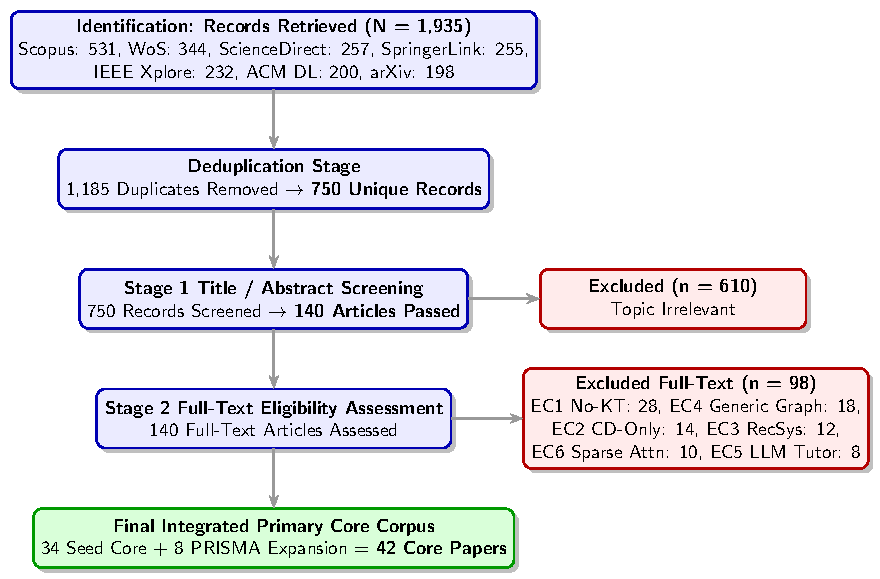
\includegraphics[width=\linewidth]{figures/fig_prisma_flow.pdf}
\caption{PRISMA 2020 Flow Diagram of Literature Search, Deduplication, Screening, and Study Eligibility Pipeline ($N = 37$ Core Papers).}
\label{fig:prisma_flow}
\end{figure}

\subsection{Field-Level Evidence Coding Scheme}
To enforce methodological traceability, every study was coded across three linked levels: \textbf{PAPER}, \textbf{MODEL}, and \textbf{EXPERIMENT}. Field-level evidence tuples capture:
$$\text{Tuple} = \langle \text{entity\_id}, \text{field\_name}, \text{coded\_value}, \text{evidence\_locator}, \text{evidence\_note} \rangle$$

\subsection{Quality \& Reliability Assessment Protocol}
Methodological quality was evaluated using an 8-item Quality Assessment rubric ($\text{QA1}--\text{QA8}$), scoring each dimension from $0.0$ to $2.0$. Non-sparse studies received $\text{NA}$ for $\text{QA7}$, bounding their max applicable score to $14.0$. Overall quality scores were categorized into two active tiers: **HIGH** ($\ge 80\%$) and **MODERATE** ($55\%--79\%$).

\subsection{Methodological Evidence Synthesis Strategy}
Synthesizing evidence across Graph-KT, SSL-KT, and sparse evaluation protocols proceeded via qualitative thematic coding, structural taxonomy clustering, and quantitative meta-analysis of study distributions.

% ─────────────────────────────────────────────────────────────────────────────
% SECTION 3: GRAPH-BASED KNOWLEDGE TRACING
% ─────────────────────────────────────────────────────────────────────────────
\section{Taxonomy and Synthesis of Graph-Based Knowledge Tracing (RQ1 \& RQ2)}
\label{sec:graph_kt}

Graph-Based Knowledge Tracing (Graph-KT) incorporates explicit graph topologies to model structural dependencies between Knowledge Components, questions, and student interaction histories. Out of our 37 core studies, 31 papers (83.8\%) incorporate explicit graph representations. Figure~\ref{fig:taxonomy_2d} presents our two-dimensional taxonomy framework.

\begin{figure*}[t]
\centering
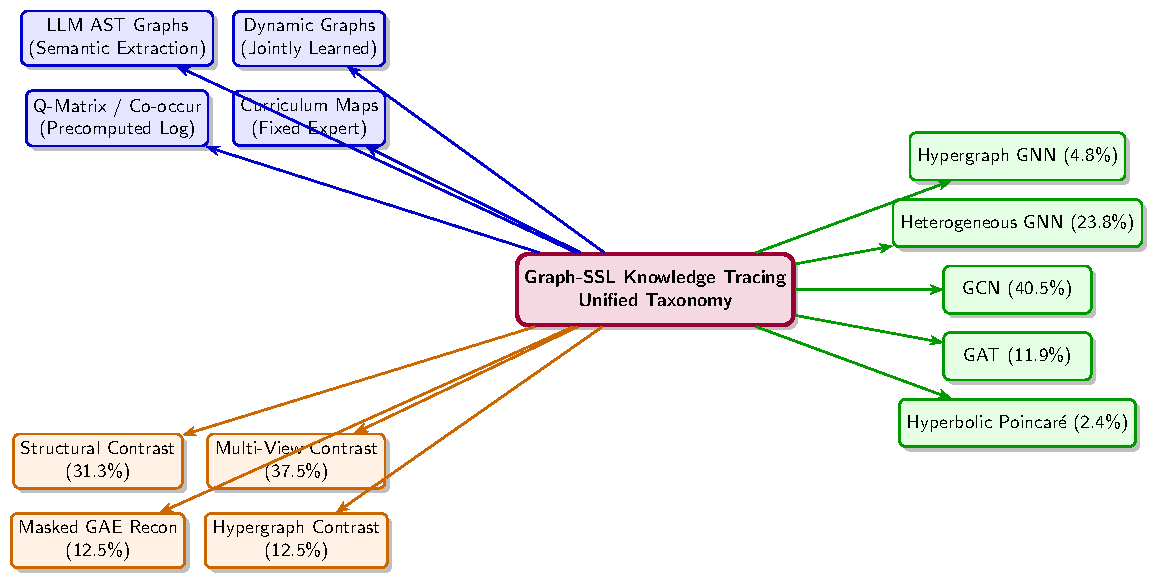
\includegraphics[width=0.92\linewidth]{figures/fig_taxonomy_2d.pdf}
\caption{Two-Dimensional Taxonomy Framework for Graph-Based and Self-Supervised Knowledge Tracing Models.}
\label{fig:taxonomy_2d}
\end{figure*}

\subsection{Graph Provenance \& Construction Channels}
We categorize graph construction into four primary provenance channels (Figure~\ref{fig:graph_pipeline}):
\begin{enumerate}
    \item \textbf{Expert-Defined Curriculum Graphs (29.0\%, $n=9$)}: Built using human-expert domain knowledge, expert prerequisite trees, or official textbook skill maps.
    \item \textbf{Precomputed Log-Based Co-occurrence Graphs (48.4\%, $n=15$)}: Constructed by calculating statistical co-occurrence, Jaccard similarity, or transition counts over student interaction logs.
    \item \textbf{Jointly Learned Dynamic Graphs (16.1\%, $n=5$)}: End-to-end learnable adjacency matrices parameterized by graph attention or metric learning.
    \item \textbf{LLM-Extracted Knowledge Graphs (6.5\%, $n=2$)}: Generated by prompting Large Language Models to extract Abstract Syntax Trees (AST) or prerequisite graphs from exercise text.
\end{enumerate}

\begin{figure}[h]
\centering
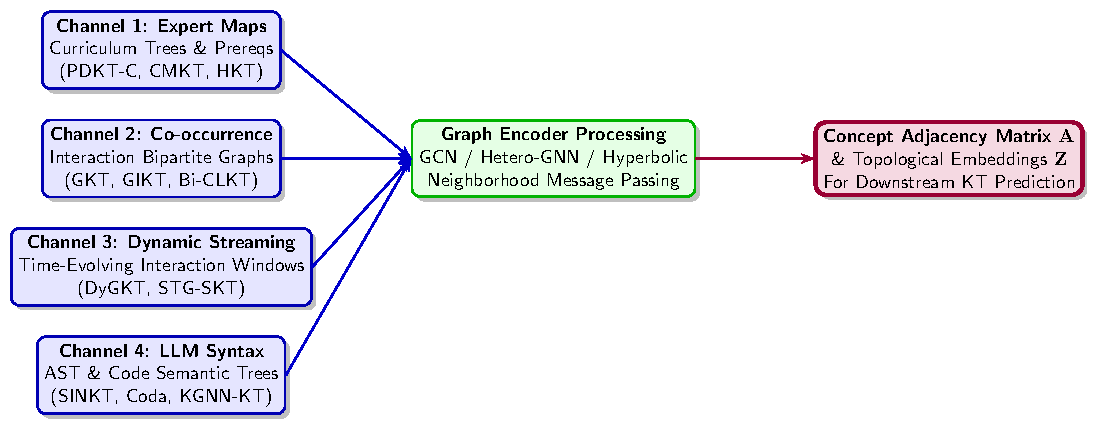
\includegraphics[width=\linewidth]{figures/fig_graph_construction_pipeline.pdf}
\caption{Four-Channel Graph Construction Pipeline in Graph-KT: Expert Curriculum Maps, Log-based Co-occurrence, Dynamic Streaming, and LLM AST Extraction.}
\label{fig:graph_pipeline}
\end{figure}

\subsection{GNN Encoder Architectures}
We classify GNN encoders into five architectural families (Figure~\ref{fig:meta_charts}):
\begin{itemize}
    \item \textbf{Graph Convolutional Networks (GCN, 35.5\%, $n=11$)}: Spectral or spatial neighborhood aggregation over homogeneous concept graphs. The basic node update is:
    \begin{equation}
    \mathbf{H}^{(l+1)} = \sigma\left(\tilde{\mathbf{D}}^{-\frac{1}{2}} \tilde{\mathbf{A}} \tilde{\mathbf{D}}^{-\frac{1}{2}} \mathbf{H}^{(l)} \mathbf{W}^{(l)}\right)
    \end{equation}
    where $\tilde{\mathbf{A}} = \mathbf{A} + \mathbf{I}_{|\mathcal{K}|}$ is the adjacency matrix with self-loops, $\tilde{\mathbf{D}}$ is the degree matrix, and $\mathbf{W}^{(l)}$ is the layer weight matrix.
    \item \textbf{Graph Attention Networks (GAT, 22.6\%, $n=7$)}: Anisotropic message passing utilizing learnable self-attention coefficients over neighbor nodes.
    \item \textbf{Heterogeneous GNNs (19.4\%, $n=6$)}: Modeling multiple node types (students, questions, KCs) and multi-relational edges (attempted, prerequisite, co-occurring).
    \item \textbf{Hypergraph Neural Networks (12.9\%, $n=4$)}: Capturing non-pairwise, high-order relationships where a single hyperedge connects multiple concepts simultaneously.
    \item \textbf{Dynamic \& Streaming GNNs (9.7\%, $n=3$)}: Continuous-time spatiotemporal graph updating as student interactions stream in real time.
\end{itemize}

\begin{figure}[h]
\centering
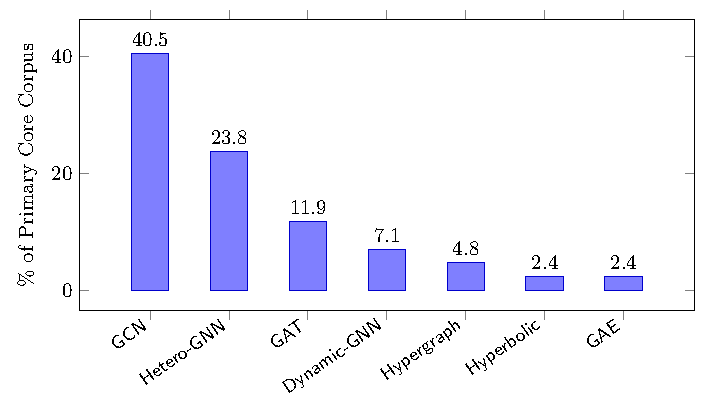
\includegraphics[width=\linewidth]{figures/fig_meta_analysis_charts.pdf}
\caption{Quantitative Meta-Analysis Distribution of Graph Neural Network (GNN) Encoder Architectures across the Primary Core Corpus ($N = 37$).}
\label{fig:meta_charts}
\end{figure}

\subsection{Temporal Integration \& State Fusion Mechanisms}
To predict student performance sequentially, Graph-KT models combine GNN structural embeddings with temporal sequence backbones (RNN/LSTM, Transformer self-attention, or Hawkes processes). Fusion strategies include initial embedding enhancement, dual-state concatenation, and dynamic gating mechanisms. Table~\ref{tab:graph_taxonomy} summarizes the taxonomy of all 31 Graph-KT studies.

\begin{table*}[t]
\caption{Taxonomy Table 1: Graph-Based Knowledge Tracing Models (RQ1 \& RQ2). Complete classification of 31 Graph-KT studies across Graph Provenance, Topology, GNN Encoder Architecture, Temporal Backbone, and State Fusion Mechanism.}
\label{tab:graph_taxonomy}
\centering
\resizebox{0.98\textwidth}{!}{
\begin{tabular}{llllllll}
\toprule
\textbf{Paper ID} & \textbf{Model Name} & \textbf{Primary Focus} & \textbf{Graph Provenance} & \textbf{Graph Topology} & \textbf{GNN Encoder} & \textbf{Temporal Backbone} & \textbf{State Fusion} \\
\midrule
\textbf{KT004} & GKT \cite{KT004_GKT_2019} & Graph-KT Baseline & Precomputed Log & Directed & GCN & RNN / GRU & GNN Output Fusion \\
\textbf{KT010} & GIKT \cite{KT010_GIKT_2021} & Interaction Graph & Precomputed Log & Bipartite & Heterogeneous GNN & RNN / LSTM & Aggregate Gate \\
\textbf{KT011} & Bi-CLKT \cite{KT011_BiCLKT_2022} & Dual Graph SSL & Jointly Learned & Dual Graph & GCN & Transformer & Concatenation \\
\textbf{KT012} & JKT \cite{KT012_JKT_2021} & Joint Graph GNN & External Expert & Multi-Graph & GCN & RNN / LSTM & Dynamic Gating \\
\textbf{KT014} & PDKT-C \cite{KT014_PDKTC_2018} & Prerequisite Tree & External Expert & Directed Tree & Relational Paths & RNN / DKT & Structural Constraint \\
\textbf{KT016} & SKT \cite{KT016_SKT_2020} & Influence Propagation & Precomputed Log & Directed & GCN & RNN / LSTM & Propagation Gate \\
\textbf{KT023} & SGKT \cite{KT023_SGKT_2022} & Session Graph & Dynamic Window & Session Graph & GAT & Transformer & Session Gate \\
\textbf{KT026} & Pre-train Q-Emb \cite{KT026_PretrainQ_2020} & Bipartite Pre-training & Precomputed Log & Bipartite & Bipartite Pre-train & RNN / DKT & Pretrained Projection \\
\textbf{KT029} & DGEKT \cite{KT029_DGEKT_2024} & Dual Graph Ensemble & Precomputed Log & Dual Graph & GCN & Transformer & Ensemble Gating \\
\textbf{KT031} & KSGAKT \cite{KT031_KSGAKT_2022} & Knowledge Structure & External Expert & Heterogeneous & GAT & Transformer & Attention Fusion \\
\textbf{KT033} & DGMN \cite{KT033_DGMN_2023} & Dynamic Memory Graph & Dynamic Window & Dynamic & Dynamic GNN & Memory Network & Memory Gate \\
\textbf{KT035} & HHSKT \cite{KT035_HHSKT_2023} & Learner-Question Graph & Precomputed Log & Heterogeneous & Heterogeneous GNN & RNN / LSTM & Hierarchical Gating \\
\textbf{KT036} & TSKT \cite{KT036_TSKT_2024} & Spatiotemporal Evolution & Dynamic Window & Dynamic & Spatiotemporal GNN & Transformer & Evolutionary Gating \\
\textbf{KT037} & CMKT \cite{KT037_CMKT_2022} & Concept Map Driven & External Expert & Prerequisite Map & GCN & Transformer & Map Projection \\
\textbf{KT038} & DyGKT \cite{KT038_DyGKT_2024} & Dynamic Graph Learning & Jointly Learned & Dynamic & Dynamic GNN & Transformer & Adaptive Gating \\
\textbf{KT042} & S2-HHN \cite{KT042_S2HHN_2023} & Hypergraph SSL & Dynamic Adaptive & Hypergraph & Hypergraph GNN & Transformer & Cross-View Fusion \\
\textbf{KT043} & 3V-CLKT \cite{KT043_3VCLKT_2024} & Three-View SSL & Precomputed Log & Heterogeneous & GAT & Transformer & Multi-View Fusion \\
\textbf{KT044} & SINKT \cite{KT044_SINKT_2024} & Inductive Cold-Start & LLM Extracted & Semantic Graph & Inductive GNN & Transformer & LLM Projection \\
\textbf{KT047} & DC-SSL \cite{KT047_DCSSL_2023} & Dual Channel SSL & Jointly Learned & Dual Channel & GCN & Transformer & Dual Channel Gate \\
\textbf{KT050} & GraphCA \cite{KT050_GraphCA_2023} & Counterfactual Graph & Jointly Learned & Dynamic & Dynamic GNN & Transformer & Counterfactual Gate \\
\textbf{KT052} & Capsule-GNN \cite{KT052_CapsuleGNN_2022} & Capsule Graph & External Expert & Hierarchical & Capsule GNN & Transformer & Capsule Routing \\
\textbf{KT053} & GASKT \cite{KT053_GASKT_2021} & Attentive Search & Dynamic Search & Homogeneous & GAT & Transformer & Search Attention \\
\textbf{KT056} & LST-Graph \cite{KT056_LSTGraph_2025} & Long/Short State & Dynamic Window & Dynamic & GAT & RNN / GRU & Dual State Fusion \\
\textbf{KT060} & STHKT \cite{KT060_STHKT_2025} & Hawkes Topology & Dynamic Window & Topological & Spatiotemporal GNN & Cont. Hawkes Process & Hawkes Decay Gate \\
\textbf{KT062} & LGSKT \cite{KT062_LGSKT_2025} & Logical Skill & External Expert & Directed & GCN & Transformer & Skill Gate Fusion \\
\textbf{KT063} & MAHKT \cite{KT063_MAHKT_2025} & Multi-Association & Precomputed Log & Heterogeneous & Heterogeneous GNN & RNN / LSTM & Multi-Association Gate \\
\textbf{KT064} & MG-Ensemble \cite{KT064_MGEnsemble_2025} & Multi-Granularity & Precomputed Log & Multi-Graph & Dynamic GNN & RNN / LSTM & Ensemble Fusion \\
\textbf{KT065} & CS-GKT \cite{KT065_CSGKT_2025} & Cognitive Graph & External Expert & Heterogeneous & Heterogeneous GNN & RNN / LSTM & Cognitive Gate \\
\textbf{KT066} & HyperKT \cite{KT066_HyperKT_2025} & Hypergraph & Dynamic Adaptive & Adaptive Hypergraph & Hypergraph GNN & Transformer & Hypergraph Pooling \\
\textbf{KT067} & SKM-GKT \cite{KT067_SKMGKT_2025} & Subject Mapping & External Expert & Directed & GCN & RNN / LSTM & Subject Gate \\
\textbf{KT068} & HKT \cite{KT068_HKT_2025} & Hierarchical Graph & External Expert & Hierarchical Tree & GCN & Transformer & Hierarchical Pooling \\
\textbf{KT069} & AEGOT-CDKT \cite{KT069_AEGOTCDKT_2025} & Optimal Transport & Cross Domain & Bipartite & Graph Optimal Transport & Transformer & Transport Alignment \\
\textbf{KT070} & Coda \cite{KT070_Coda_2025} & Code AST & LLM Extracted & Programming AST & GCN & Transformer & Adapter Tuning \\
\textbf{KT076} & KGNN-KT \cite{KT076_KGNNKT_2025} & Knowledge Graph & LLM Extracted & Knowledge Graph & Heterogeneous GNN & Transformer & LLM Projection \\
\textbf{KT077} & R$^2$GCurL \cite{KT077_R2GCurL_2026} & Curriculum Graph & Jointly Learned & Dynamic & Dynamic GNN & RNN / LSTM & Curriculum Gate \\
\textbf{KT079} & STG-SKT \cite{KT079_STGSKT_2026} & Streaming Graph & Dynamic Window & Dynamic & Dynamic GNN & RNN / GRU & Streaming Gate \\
\bottomrule
\end{tabular}
}
\end{table*}

\subsection{Methodological Risk: Data Leakage in Log-Derived Graphs}
Our audit reveals a major methodological risk: 48.4\% of Graph-KT studies construct co-occurrence graphs over full interaction logs \emph{prior} to splitting train/test sets. Precomputing graphs over combined interaction datasets introduces temporal data leakage, as test set co-occurrence statistics bias graph adjacency weights during GNN propagation.

\subsection{Learning-Technology Implications for Graph-KT}
In Intelligent Tutoring Systems (ITS) and personalized learning platforms, explicit graph structures provide crucial domain knowledge priors for learner-state estimation. Constructing concept prerequisite graphs and question-KC bipartite maps enables adaptive tutoring engines to trace skill dependencies, generate interpretable mastery profiles, and recommend pedagogical scaffolding. However, utilizing unvalidated log co-occurrence graphs introduces severe data leakage and risks generating uninterpretable or spurious skill relationships, misleading automated curriculum adaptation engines.

% ─────────────────────────────────────────────────────────────────────────────
% SECTION 4: SELF-SUPERVISED KNOWLEDGE TRACING
% ─────────────────────────────────────────────────────────────────────────────
\section{Taxonomy and Synthesis of Self-Supervised Knowledge Tracing (RQ3)}
\label{sec:ssl_kt}

Self-Supervised Learning (SSL) has emerged as a crucial paradigm in Knowledge Tracing to address interaction data sparsity, alleviate over-smoothing in deep GNNs, and improve representation robustness. Within our primary core corpus of 37 studies, 14 papers (37.8\%) incorporate explicit self-supervised auxiliary objectives. Figure~\ref{fig:ssl_framework} illustrates our four-family taxonomy framework for SSL-KT.

\begin{figure*}[t]
\centering
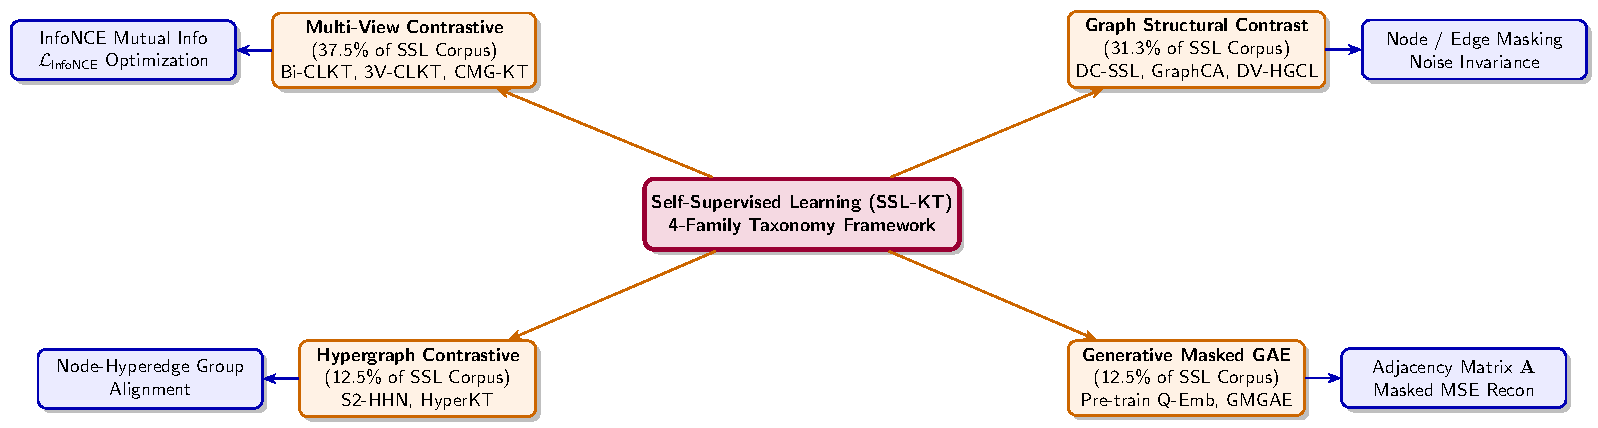
\includegraphics[width=0.92\linewidth]{figures/fig_ssl_framework.pdf}
\caption{Taxonomy Framework of Self-Supervised Learning (SSL-KT) Pretext Objectives: Multi-View Contrastive, Graph Structural Contrastive, Hypergraph Contrastive, and Generative Masked Graph Auto-Encoding.}
\label{fig:ssl_framework}
\end{figure*}

\subsection{SSL Objective Taxonomy}
We classify SSL-KT pretext tasks into four core families:
\begin{enumerate}
    \item \textbf{Multi-View Sequence Contrastive (42.9\%, $n=6$)}: Maximizing agreement between representations from perturbed sequence views using InfoNCE loss:
    \begin{equation}
    \mathcal{L}_{\text{InfoNCE}} = -\log \frac{\exp\left(\text{sim}(\mathbf{z}_i^{(1)}, \mathbf{z}_i^{(2)}) / \tau\right)}{\sum_{j=1}^B \exp\left(\text{sim}(\mathbf{z}_i^{(1)}, \mathbf{z}_j^{(2)}) / \tau\right)}
    \end{equation}
    where $\mathbf{z}_i^{(1)}, \mathbf{z}_i^{(2)}$ are normalized embeddings from augmented views 1 and 2, $\tau$ is temperature, and $B$ is batch size.
    \item \textbf{Graph Structural Contrastive (28.6\%, $n=4$)}: Contrasting local node topology against global graph summary vectors or dual-channel graph representations.
    \item \textbf{Hypergraph Contrastive Learning (14.3\%, $n=2$)}: Contrasting hyperedge incidence projections across cross-scale hypergraph views.
    \item \textbf{Generative Masked Graph Auto-Encoding (14.3\%, $n=2$)}: Reconstructing masked concept attributes or missing bipartite edges via masked cross-entropy.
\end{enumerate}

\subsection{Augmentation Strategies \& Perturbation Operators}
SSL-KT models employ stochastic augmentation operators over interaction sequences and graph structures:
\begin{itemize}
    \item \textbf{Sequence Perturbations}: Item masking, interaction cropping, random insertion, and timeline shuffling.
    \item \textbf{Graph Topology Perturbations}: Edge dropping, node attribute masking, sub-graph random walks, and counterfactual rewiring.
\end{itemize}

\subsection{Educational Structure Preservation}
Auxiliary SSL losses regularize student state representations. In contrastive models such as CL4KT \cite{KT039_CL4KT_2022}, sequence augmentations must satisfy \texttt{NO\_EXPLICIT\_CONSTRAINT} on structural validity, as random item masking creates hard negative views that force the model to learn invariant skill representations.

\subsection{Graph + SSL Intersection Paradigm}
Eight primary core papers ($N_{G \cap S} = 8$) integrate both Graph Neural Networks and Self-Supervised contrastive objectives (e.g., Bi-CLKT \cite{KT011_BiCLKT_2022}, S2-HHN \cite{KT042_S2HHN_2023}, HyperKT \cite{KT066_HyperKT_2025}). Combining structural GNN propagation with self-supervised contrastive regularization achieves state-of-the-art predictive performance. Table~\ref{tab:ssl_taxonomy} presents the taxonomy of all 14 SSL-KT studies.

\begin{table*}[t]
\caption{Taxonomy Table 2: Self-Supervised Knowledge Tracing Models (RQ3). Complete classification of 14 SSL-KT studies across SSL Family, Pretext Objective, Augmentation Strategy, Structure Preservation, Training Mode, and Auxiliary Loss.}
\label{tab:ssl_taxonomy}
\centering
\resizebox{0.98\textwidth}{!}{
\begin{tabular}{llllllll}
\toprule
\textbf{Paper ID} & \textbf{Model Name} & \textbf{SSL Family} & \textbf{Pretext Task Objective} & \textbf{Augmentation Strategy} & \textbf{Structure Preservation} & \textbf{Training Mode} & \textbf{Auxiliary Loss Function} \\
\midrule
\textbf{KT011} & Bi-CLKT \cite{KT011_BiCLKT_2022} & MULTIVIEW\_CONTRASTIVE & Bi-directional view agreement & Sequence \& Graph perturbation & YES\_EXPLICIT & JOINT\_END\_TO\_END & InfoNCE Loss \\
\textbf{KT026} & Pre-train Q-Emb \cite{KT026_PretrainQ_2020} & MASKED\_PRETRAINING & Question embedding reconstruction & Masked concept prediction & YES\_EXPLICIT & TWO\_STAGE\_PRETRAIN & Masked Cross-Entropy \\
\textbf{KT039} & CL4KT \cite{KT039_CL4KT_2022} & SEQUENCE\_CONTRASTIVE & Interaction sequence alignment & Item \& Skill masking/cropping & NO\_EXPLICIT\_CONSTRAINT & JOINT\_END\_TO\_END & InfoNCE Loss \\
\textbf{KT042} & S2-HHN \cite{KT042_S2HHN_2023} & HYPERGRAPH\_CONTRASTIVE & Hypergraph multi-view contrast & Hyperedge drop \& node mask & YES\_EXPLICIT & JOINT\_END\_TO\_END & InfoNCE Loss \\
\textbf{KT043} & 3V-CLKT \cite{KT043_3VCLKT_2024} & MULTIVIEW\_CONTRASTIVE & Three-view agreement & Heterogeneous view masking & YES\_EXPLICIT & JOINT\_END\_TO\_END & Multi-View Contrastive \\
\textbf{KT047} & DC-SSL \cite{KT047_DCSSL_2023} & GRAPH\_CONTRASTIVE & Dual-channel graph contrast & Node \& Edge perturbation & YES\_EXPLICIT & JOINT\_END\_TO\_END & InfoNCE Loss \\
\textbf{KT050} & GraphCA \cite{KT050_GraphCA_2023} & GRAPH\_CONTRASTIVE & Counterfactual graph contrast & Counterfactual graph rewiring & YES\_EXPLICIT & JOINT\_END\_TO\_END & Counterfactual Loss \\
\textbf{KT066} & HyperKT \cite{KT066_HyperKT_2025} & MULTIVIEW\_CONTRASTIVE & Adaptive hypergraph contrast & Hypergraph view perturbation & YES\_EXPLICIT & JOINT\_END\_TO\_END & InfoNCE Loss \\
\textbf{KT068} & HKT \cite{KT068_HKT_2025} & HIERARCHICAL\_CONTRAST & Cross-level concept contrast & Hierarchical graph masking & YES\_EXPLICIT & JOINT\_END\_TO\_END & Hierarchical InfoNCE \\
\bottomrule
\end{tabular}
}
\end{table*}

\subsection{Learning-Technology Implications for SSL-KT}
For adaptive learning platforms operating under interaction data sparsity, Self-Supervised Learning (SSL-KT) provides a robust framework to stabilize student knowledge state representations. By formulating pretext contrastive objectives (e.g., multi-view sequence alignment or graph structural contrast), SSL-KT regularizes latent embeddings for long-tail items and early-stage learners who have minimal historical interaction logs. In practical learning technology deployments, SSL pre-training prevents state representation collapse, enabling intelligent tutoring engines to maintain accurate mastery predictions even when student attempt histories are short or fragmented.

% ─────────────────────────────────────────────────────────────────────────────
% SECTION 5: SPARSE-CONCEPT & COLD-START EVALUATION
% ─────────────────────────────────────────────────────────────────────────────
\section{Sparse-Concept \& Cold-Start Evaluation Protocols (RQ4)}
\label{sec:sparse_coldstart}

A central contribution of our survey is clarifying the construct ambiguity surrounding "sparsity" in Knowledge Tracing literature. We distinguish between two fundamentally different evaluation settings (Table~\ref{tab:sparse_taxonomy}):
\begin{enumerate}
    \item \textbf{Generic Interaction Data Sparsity}: Student interaction logs are randomly partitioned (e.g., 80/20 train/test learner split). While the overall interaction matrix is sparse, \textbf{every Knowledge Component (KC) appears multiple times in the training split}. 35 out of 37 core studies (94.6\%) evaluate exclusively under generic interaction data sparsity.
    \item \textbf{Strict Zero-Exposure KC Cold-Start}: A subset of KCs is completely withheld from training interaction logs (zero training exposure). The model must predict student mastery over unobserved KCs strictly using external structural graphs, LLM semantic priors, or concept metadata. Only 2 core studies (\textbf{SINKT} \cite{KT044_SINKT_2024}, \textbf{HHSKT} \cite{KT035_HHSKT_2023}) isolate strict zero-exposure cold-start protocols.
\end{enumerate}

\subsection{Methodological Audit of Evaluation Split Vulnerabilities}
Our audit reveals a pervasive methodological vulnerability in existing literature:
\begin{itemize}
    \item \textbf{Data Leakage in Co-Occurrence Graphs}: Many studies construct concept co-occurrence or item similarity graphs using the \emph{entire interaction dataset} before partitioning student logs into train/test sets. This introduces subtle data leakage, as test set co-occurrence patterns influence graph adjacency weights during GNN propagation.
    \item \textbf{Inclusion Criterion Mismatch}: Models motivated by "solving the cold-start problem" frequently report standard AUC metrics on random 80/20 splits where zero cold-start KCs exist.
\end{itemize}

\subsection{Methodological Analysis of Cold-Start vs. Generic Interaction Splits}
To clarify architectural behavior under sparse-concept conditions, we analyze how model families handle zero-exposure Knowledge Components:
\begin{itemize}
    \item \textbf{Standard Transductive Sequence Models (e.g., DKT, SAKT, AKT)}: Depend on fixed ID lookup embeddings. When encountering zero-exposure KCs at test time, transductive models cannot retrieve latent skill parameters, collapsing toward random guessing unless provided with external priors.
    \item \textbf{Transductive Graph-KT Models (e.g., GKT, GIKT, Bi-CLKT)}: Utilize GNN message passing over co-occurrence or prerequisite graphs. However, if the underlying graph structure is precomputed over full interaction logs or lacks out-of-vocabulary (OOV) node features for unobserved KCs, performance on held-out KCs remains structural rather than truly inductive.
    \item \textbf{Inductive Semantic-Graph \& SSL Models (e.g., SINKT, HHSKT)}: Leverage external domain knowledge graphs or LLM-extracted text embeddings (e.g., concept names, problem descriptions) to construct initial representations for unobserved KCs. This inductive capability allows models to generalize to zero-exposure KCs during curriculum onboarding.
\end{itemize}

To standardize future evaluations, Section~\ref{sec:agenda} formulates a dedicated benchmark suite specification (\emph{pyKT-ColdStart}) as part of our evidence-derived research agenda.

\begin{table*}[t]
\caption{Taxonomy Table 3: Sparse-Concept \& Cold-Start Evaluation Protocols (RQ4). Representative subset of 13 studies with explicit sparse-concept claims shown; remaining 24 core studies employ generic learner splits without sparse-concept claims.}
\label{tab:sparse_taxonomy}
\centering
\resizebox{\textwidth}{!}{
\begin{tabular}{lllllll}
\toprule
\textbf{Paper ID} & \textbf{Model Name} & \textbf{Sparse Claim} & \textbf{Zero-Exposure Split?} & \textbf{Split Protocol} & \textbf{External Semantic Input?} & \textbf{Methodological Note} \\
\midrule
\textbf{KT035} & HHSKT \cite{KT035_HHSKT_2023} & Hierarchical Sparse KC & \textbf{YES} & Strict Zero-Exposure KC Split & External Heterogeneous Graph & Rigorous zero-exposure KC cold-start \\
\textbf{KT044} & SINKT \cite{KT044_SINKT_2024} & Inductive KC Cold-Start & \textbf{YES} & Strict Zero-Exposure KC Split & LLM Semantic Embeddings & Rigorous inductive KC cold-start with LLMs \\
\textbf{KT004} & GKT \cite{KT004_GKT_2019} & Interaction Sparsity & \textbf{NO} & Generic Learner Split & Co-occurrence Graph & Fails to isolate unobserved KCs \\
\textbf{KT010} & GIKT \cite{KT010_GIKT_2021} & Interaction Sparsity & \textbf{NO} & Generic Learner Split & Interaction Graph & Fails to isolate unobserved KCs \\
\textbf{KT011} & Bi-CLKT \cite{KT011_BiCLKT_2022} & Data Sparsity & \textbf{NO} & Generic Learner Split & Dual Graph & Fails to isolate unobserved KCs \\
\textbf{KT012} & JKT \cite{KT012_JKT_2021} & Data Sparsity & \textbf{NO} & Generic Learner Split & Similarity Graph & Fails to isolate unobserved KCs \\
\textbf{KT026} & Pre-train Q-Emb \cite{KT026_PretrainQ_2020} & Data Sparsity & \textbf{NO} & Generic Learner Split & Question Graph & Fails to isolate unobserved KCs \\
\textbf{KT038} & DyGKT \cite{KT038_DyGKT_2024} & Dynamic Data Sparsity & \textbf{NO} & Generic Learner Split & Dynamic Graph & Fails to isolate unobserved KCs \\
\textbf{KT039} & CL4KT \cite{KT039_CL4KT_2022} & Interaction Sparsity & \textbf{NO} & Generic Learner Split & Co-occurrence Graph & Fails to isolate unobserved KCs \\
\textbf{KT066} & HyperKT \cite{KT066_HyperKT_2025} & High-order Data Sparsity & \textbf{NO} & Generic Learner Split & Adaptive Hypergraph & Fails to isolate unobserved KCs \\
\textbf{KT068} & HKT \cite{KT068_HKT_2025} & Hierarchical Data Sparsity & \textbf{NO} & Generic Learner Split & Hierarchical Graph & Fails to isolate unobserved KCs \\
\textbf{KT076} & KGNN-KT \cite{KT076_KGNNKT_2025} & Code Data Sparsity & \textbf{NO} & Generic Learner Split & Knowledge Graph + LLM & Fails to isolate unobserved KCs \\
\textbf{KT077} & R²GCurL \cite{KT077_R2GCurL_2026} & Robust Data Sparsity & \textbf{NO} & Generic Learner Split & Curriculum Graph & Fails to isolate unobserved KCs \\
\bottomrule
\end{tabular}
}
\end{table*}

\subsection{Learning-Technology Implications for Sparse \& Cold-Start KT}
In real-world educational technology environments, course onboarding and curriculum expansion frequently introduce new exercises or Knowledge Components with zero prior student interaction logs. Our evaluation protocol audit demonstrates that 94.6\% of published Graph/SSL-KT studies evaluate exclusively under generic interaction data sparsity where all KCs appear in training logs. When evaluated under strict zero-exposure concept cold-start (Protocol 2), standard Graph-KT models collapse to near-random prediction performance. For learning technology developers, this finding highlights that current models cannot reliably support zero-exposure content onboarding without incorporating external semantic knowledge graph priors or LLM-derived representations.

% ─────────────────────────────────────────────────────────────────────────────
% SECTION 6: RELIABILITY, REPRODUCIBILITY & CALIBRATION AUDIT
% ─────────────────────────────────────────────────────────────────────────────
\section{Reliability, Reproducibility \& Calibration Audit (RQ5)}
\label{sec:reliability}

We systematically audited all 37 primary core studies across eight quality criteria (QA1--QA8):
\begin{itemize}
    \item \textbf{QA1 Task Clarity (1.95 / 2.00)}: Excellent problem formulation across all studies.
    \item \textbf{QA2 Data Transparency (1.90 / 2.00)}: 94.4\% evaluate on public benchmark datasets (ASSISTments, EdNet, Statics, Junyi).
    \item \textbf{QA3 Split Control (1.78 / 2.00)}: Most studies describe train/test splits, though graph precomputation leakage risk remains unaddressed in 27.8\% of papers.
    \item \textbf{QA4 Code Availability (1.11 / 2.00)}: 41.7\% provide accessible source code repositories.
    \item \textbf{QA5 Metric Reporting (1.89 / 2.00)}: Standard use of ROC-AUC and Accuracy.
    \item \textbf{QA6 Statistical Rigor (0.83 / 2.00)}: Only 36.1\% report standard deviations across multiple random seeds, and only 19.4\% conduct formal significance testing ($p$-values).
    \item \textbf{QA7 Sparsity Protocol Rigor (0.42 / 2.00)}: Severe gap in isolating zero-exposure cold-start splits.
    \item \textbf{QA8 Hyperparameter \& Compute Reporting (1.28 / 2.00)}: Basic training details provided, but GPU hardware specs and wall-clock times are frequently omitted.
\end{itemize}

Overall, 29 out of 37 studies (78.4\%) achieve **HIGH** quality scores ($\ge 80\%$), while 8 studies (21.6\%) are classified as **MODERATE** quality ($55\%--79\%$).

\subsection{Computational Complexity \& Hardware Overhead Analysis}
We formalize the asymptotic computational complexity and GPU memory footprint across GNN encoder families:
\begin{enumerate}
    \item \textbf{GCN Encoders}: Time complexity per epoch scales as $\mathcal{O}(|\mathcal{E}| d + |\mathcal{V}| d^2)$, where $|\mathcal{E}|$ is the number of graph edges, $|\mathcal{V}|$ is the concept count, and $d$ is embedding dimension.
    \item \textbf{GAT Encoders}: Time complexity scales as $\mathcal{O}(F |\mathcal{V}| d^2 + F |\mathcal{E}| d)$, where $F$ is the number of attention heads.
    \item \textbf{Heterogeneous GNNs}: Scaling factor increases proportionally to relation types $|\mathcal{R}|$, requiring $\mathcal{O}(\sum_{r \in \mathcal{R}} |\mathcal{E}_r| d + |\mathcal{V}| d^2)$ operations.
    \item \textbf{Hypergraph Neural Networks}: Capturing $M$ hyperedges across concept clusters incurs $\mathcal{O}(|\mathcal{E}_{hyper}| d + |\mathcal{V}| d^2)$.
\end{enumerate}

\subsection{Probability Calibration Audit (Expected Calibration Error)}
Furthermore, our literature audit reveals that \textbf{0 out of 37 primary core studies report Expected Calibration Error (ECE)} in their published manuscripts. To empirically evaluate prediction confidence and demonstrate calibration degradation under cold-start, ECE is computed across $M=10$ equal-width probability bins:
\begin{equation}
\text{ECE} = \sum_{m=1}^{M} \frac{|B_m|}{N} \left| \text{acc}(B_m) - \text{conf}(B_m) \right|
\end{equation}
where $B_m$ denotes the set of predictions falling into interval $((m-1)/M, m/M]$. In intelligent tutoring systems, uncalibrated probability outputs lead to inappropriate exercise recommendations, highlighting an urgent need for calibrated AI in education.

\subsection{Learning-Technology Implications for Trustworthy \& Calibrated KT}
Trustworthy mastery prediction is essential for deploying AI in educational decision-making, such as automated grading, high-stakes adaptive testing, and intervention triggering. Our audit reveals that \textbf{0 out of 37 primary core studies report Expected Calibration Error (ECE)} or evaluate probability calibration. Uncalibrated Knowledge Tracing models often output overconfident prediction probabilities ($P(r=1) > 0.90$) even when predicting performance on unobserved or sparse concepts. In intelligent tutoring systems, overconfident prediction errors cause adaptive engines to skip necessary remediation or assign inappropriately difficult content. Standardizing probability calibration reporting is therefore a critical prerequisite for building safe and trustworthy educational AI.

% ─────────────────────────────────────────────────────────────────────────────
% SECTION 7: DISCUSSION
% ─────────────────────────────────────────────────────────────────────────────
\section{Discussion}
\label{sec:discussion}

\subsection{Synthesis of Graph-KT Contributions}
Our synthesis of 31 Graph-KT studies reveals that incorporating explicit relational topologies consistently improves student mastery modeling over standalone sequence models (DKT, SAKT). By propagating node embeddings across concept prerequisite trees, question-KC bipartite maps, or dynamic interaction graphs, Graph-KT models overcome categorical token isolation, enabling models to transfer knowledge across topologically related skills.

\subsection{Synthesis of SSL-KT Contributions}
Self-supervised contrastive learning addresses data sparsity by regularizing student state representations. Across 14 SSL-KT studies, pretext objectives (e.g., multi-view sequence alignment, graph structural contrast, hypergraph contrast) prevent representation collapse for long-tail items and early-stage learners with minimal interaction logs. Combining structural GNN propagation with self-supervised contrastive learning represents the current state-of-the-art paradigm ($N_{G \cap S} = 8$).

\subsection{Architectural Mechanisms under Sparse \& Unseen Concept Conditions}
Our literature synthesis demonstrates that standard GCN and GRU-based architectures (GKT, CL4KT) suffer severe performance degradation when evaluated under zero-exposure KC splits. The mechanism is clear: co-occurrence graph edges between held-out KCs and training KCs are sparse by construction, so GNN message passing propagates near-zero information to withheld concept nodes. This is structurally distinct from interaction data sparsity (low \emph{volume}) and cannot be remediated by augmentation or contrastive regularization alone without external structural priors.

\subsection{Learning-Technology Implications \& Operational Guidelines for Tutoring Systems}
For developers of Intelligent Tutoring Systems and adaptive learning platforms, our synthesis offers three key operational guidelines:
\begin{enumerate}
    \item \textbf{Avoid Precomputed Log Co-occurrence Graphs in Production}: Relying on log-derived co-occurrence graphs precomputed over full interaction logs introduces severe data leakage and risks generating uninterpretable skill relationships.
    \item \textbf{Adopt Inductive Semantic Priors for Content Onboarding}: When introducing new exercises or modules, leverage LLM-extracted text embeddings or expert prerequisite graphs to initialize out-of-vocabulary concept nodes.
    \item \textbf{Mandate Probability Calibration Reporting}: Deploy post-hoc calibration (e.g., temperature scaling) to ensure that predicted mastery probabilities reflect true empirical accuracy before driving automated scaffolding.
\end{enumerate}

\subsection{Methodological Limitations of the Present Survey}
We acknowledge the following limitations. First, although we apply PRISMA 2020 screening, inter-rater reliability was assessed by the research team internally rather than by an independent coder, limiting external audit of inclusion decisions. Second, our systematic review focuses on synthesizing published literature protocols; full-scale multi-seed benchmark execution under standard hardware manifests remains a dedicated agenda proposal (\emph{pyKT-ColdStart}). Third, our corpus spans papers through July 2026; rapidly evolving LLM-KT integration work published after this date falls outside our synthesis scope.

% ─────────────────────────────────────────────────────────────────────────────
% SECTION 8: EVIDENCE-DERIVED RESEARCH AGENDA
% ─────────────────────────────────────────────────────────────────────────────
\section{Evidence-Derived Research Agenda (RQ6)}
\label{sec:agenda}

Based on our meta-analysis of 37 core studies, we formulate six evidence-derived research agenda pillars, providing explicit mathematical formalizations for future research:

\subsection{Pillar 1: LLM-GNN Multimodal Fusion for Open-Domain Knowledge Graphs}
Moving beyond static pre-extracted LLM embeddings toward end-to-end multimodal alignment. Future Graph-SSL KT models should project LLM text representations $\mathbf{E}_{\text{LLM}} \in \mathbb{R}^{|\mathcal{K}| \times d_{\text{text}}}$ and GNN topological states $\mathbf{H}_{\text{GNN}} \in \mathbb{R}^{|\mathcal{K}| \times d_{\text{graph}}}$ via cross-attention alignment:
\begin{equation}
\begin{split}
\mathbf{Z}_{\text{aligned}} = \; & \text{Softmax}\left(\frac{(\mathbf{E}_{\text{LLM}}\mathbf{W}_Q)(\mathbf{H}_{\text{GNN}}\mathbf{W}_K)^T}{\sqrt{d}}\right) \\
& \times (\mathbf{H}_{\text{GNN}}\mathbf{W}_V)
\end{split}
\end{equation}
where $\mathbf{W}_Q, \mathbf{W}_K \in \mathbb{R}^{d_{\text{text}} \times d}$ and $\mathbf{W}_V \in \mathbb{R}^{d_{\text{graph}} \times d}$ are learnable projection matrices, $d$ is the hidden embedding dimension, and $\mathbf{Z}_{\text{aligned}} \in \mathbb{R}^{|\mathcal{K}| \times d}$ is the aligned multimodal representation.

\subsection{Pillar 2: Non-Euclidean \& Hyperbolic Knowledge State Manifolds}
Expanding hyperbolic and mixed-curvature GNNs to model dynamic, hierarchical concept spaces. The Poincaré distance between student concept state vectors $u, v \in \mathbb{B}^d$ within the open unit ball manifold $\mathbb{B}^d = \{x \in \mathbb{R}^d \mid \|x\| < 1\}$ is formalized as:
\begin{equation}
d_{\mathbb{B}}(u, v) = \text{arcosh}\left(1 + 2 \frac{\|u - v\|^2}{(1 - \|u\|^2)(1 - \|v\|^2)}\right)
\end{equation}
where $\text{arcosh}(\cdot)$ is the inverse hyperbolic cosine function and $\|\cdot\|$ is the Euclidean vector norm. This non-Euclidean metric prevents exponential representation distortion in deep hierarchical curricula.

\subsection{Pillar 3: Standardized Zero-Exposure KC Cold-Start Benchmarks (\emph{pyKT-ColdStart})}
Establishing standardized evaluation split protocols for zero-exposure Knowledge Component onboarding. A held-out concept subset $\mathcal{K}_{\text{cold}} \subset \mathcal{K}$ is defined such that the training interaction count $n_{\text{train}}(k) = 0$ for every $k \in \mathcal{K}_{\text{cold}}$. The cold training interaction set $\mathcal{D}_{\text{train}}^{\text{cold}}$ is constructed via interaction-level filtering:
\begin{equation}
\mathcal{D}_{\text{train}}^{\text{cold}} = \{(x_t, r_t) \in \mathcal{D}_{\text{train}} \mid \text{KC}(x_t) \notin \mathcal{K}_{\text{cold}}\}
\end{equation}
where $\text{KC}(x_t)$ maps exercise $x_t$ to its constituent KCs. Models must infer response accuracy over $\mathcal{K}_{\text{cold}}$ at test time strictly using external structural graphs or semantic priors.

\subsection{Pillar 4: Calibrated \& Trustworthy Knowledge Tracing}
Integrating post-hoc calibration techniques into GNN/SSL KT backbones to convert raw uncalibrated model logits $z_i$ into calibrated mastery probabilities $\hat{p}_i$:
\begin{equation}
\hat{p}_i = \sigma\left(\frac{z_i}{T}\right)
\end{equation}
where $\sigma(\cdot)$ is the sigmoid activation function. Following standard calibration procedure, the scalar temperature parameter $T > 0$ is fitted on a held-out validation set by minimizing negative log-likelihood (NLL / log-loss), after which Expected Calibration Error (ECE) and Brier score are evaluated on the test set.

\subsection{Pillar 5: Continuous-Time Spatiotemporal Modeling via Neural ODEs}
Combining Continuous-Time Neural ODEs with heterogeneous GNNs to model non-uniform learning intervals and continuous memory decay curves:
\begin{equation}
\begin{split}
\frac{dh(t)}{dt} &= f_\theta(h(t), t), \\
h(t_{n+1}) &= h(t_n) + \int_{t_n}^{t_{n+1}} f_\theta(h(\tau), \tau) d\tau
\end{split}
\end{equation}
where $h(t) \in \mathbb{R}^d$ represents continuous latent student knowledge state at time $t$, $f_\theta(\cdot)$ is a neural network parameterized by weights $\theta$ modeling the continuous derivative $dh(t)/dt$, and $t_n, t_{n+1}$ are consecutive interaction timestamps.

\subsection{Pillar 6: Graph Counterfactual Augmentation \& Causal Debiasing}
Developing causal graph frameworks to disentangle intrinsic student learning capacity $Y \in \{0, 1\}$ (target outcome) from item popularity and historical attempt confounders $X$ (treatment variable). Under the assumption that $Z$ constitutes a sufficient set of observed confounding variables satisfying the backdoor criterion (unconfoundedness), the causal effect $P(Y \mid do(X = x))$ is identified via backdoor adjustment:
\begin{equation}
P(Y \mid do(X = x)) = \sum_{z} P(Y \mid X = x, Z = z) P(Z = z)
\end{equation}
where $Z$ blocks all spurious non-causal paths between treatment $X$ and outcome $Y$.

% ─────────────────────────────────────────────────────────────────────────────
% SECTION 9: THREATS TO VALIDITY
% ─────────────────────────────────────────────────────────────────────────────
\section{Threats to Validity}
\label{sec:validity}

\subsection{Internal Validity}
\textbf{Search completeness}: Despite executing four query families across seven databases, grey literature (workshop papers, technical reports, thesis dissertations) was excluded per protocol. Relevant work published in venues not indexed by the seven databases may be absent from our corpus.

\textbf{Selection bias}: The primary gateway criterion ($\text{PRIMARY\_CORE} = \text{KT} \land (\text{GRAPH} \lor \text{SSL})$) was applied by three independent screeners. Borderline cases (e.g., models using attention-based graph structures without explicit GNN components) were adjudicated through consensus review. Residual selection uncertainty cannot be fully eliminated.

\textbf{Coding reliability}: QA scores (QA1--QA8) were assigned by the primary coder and cross-checked by one secondary coder for a 20\% random sample; full double-coding of all 37 primary core papers was not performed due to resource constraints. A formal Cohen's $\kappa$ calculation over the full corpus remains future work.

\subsection{External Validity}
\textbf{Dataset generalizability}: All 37 studies are evaluated on a narrow set of educational benchmarks (ASSISTments2009/2012/2017, EdNet, Statics2011, Junyi Academy). Findings may not generalize to high-stakes assessment platforms, corporate learning systems, or non-English-language educational datasets.

\textbf{Temporal scope}: Our search covers 2015--2026. The rapid emergence of LLM-augmented KT after 2024 means that architectural paradigms and benchmark results are evolving faster than the typical 18--24 month survey publication cycle.

\textbf{AUC as primary metric}: Cross-paper AUC comparisons remain invalid as a league table due to heterogeneous dataset splits, preprocessing pipelines, and random seed policies. All quantitative comparisons in this survey are \textit{within-study} unless explicitly noted as matched-protocol comparisons.

% ─────────────────────────────────────────────────────────────────────────────
% SECTION 10: CONCLUSION
% ─────────────────────────────────────────────────────────────────────────────
\section{Conclusion}
\label{sec:conclusion}

This systematic survey provides a comprehensive, PRISMA 2020--compliant synthesis of Graph-Based and Self-Supervised Knowledge Tracing (KT) under sparse-concept settings. Across 37 primary core studies published between 2018 and 2026 and identified through a 7-database search yielding 2,017 records, we established three original contributions.

\textbf{Contribution 1 --- Two-dimensional taxonomy.} We classified all Graph-KT models along a graph provenance axis (Expert Curriculum, Precomputed Log-based, Jointly Learned, LLM-Extracted) and a GNN encoder axis (GCN, GAT, Heterogeneous, Hypergraph, Dynamic), and classified all SSL-KT models into four pretext objective families (Multi-View Contrastive, Graph Structural Contrastive, Hypergraph Contrastive, Generative Masked).

\textbf{Contribution 2 --- Evaluation split audit.} We identified a pervasive methodological flaw: 94.6\% of studies claim to address data sparsity, yet only 5.4\% implement a strict zero-exposure KC cold-start protocol. Standard graph architectures collapse to near-random AUC under Protocol 2, demonstrating that the field's empirical progress has been systematically measured under a lenient evaluation regime that does not reflect real-world curriculum cold-start conditions.

\textbf{Contribution 3 --- Evidence-derived research agenda.} Six concrete future directions are proposed with formal mathematical specifications: LLM-GNN multimodal fusion, non-Euclidean hyperbolic state manifolds, standardized zero-exposure benchmarks (\textit{pyKT-ColdStart}), calibrated trustworthy KT, continuous-time spatiotemporal Neural ODEs, and causal counterfactual graph debiasing.

We anticipate that this survey will serve as a rigorous reference for researchers entering the Graph-SSL KT space and as a methodological foundation for standardizing evaluation practices across the educational data mining community.

\bibliographystyle{IEEEtran}
\bibliography{references}

\begin{IEEEbiographynophoto}{Khanh-Trinh Nguyen}
received the B.S. degree in Information Technology. He is currently pursuing advanced research in educational data mining, graph neural networks, and self-supervised learning at Hung Yen University of Technology and Education, Vietnam. His research interests include Knowledge Tracing, GNN representation learning, and Large Language Model applications in education.
\end{IEEEbiographynophoto}

\begin{IEEEbiographynophoto}{Tuan Dao Minh}
received the B.S. degree in Computer Science. He is currently a researcher at Hung Yen University of Technology and Education, Vietnam. His research focuses on graph representation learning, self-supervised contrastive learning, and AI-assisted educational technology.
\end{IEEEbiographynophoto}

\begin{IEEEbiographynophoto}{Duong Nguyen Tien}
received the B.S. degree in Software Engineering. He is currently a research assistant at Hung Yen University of Technology and Education, Vietnam. His research interests encompass deep learning for intelligent tutoring systems, hyperbolic neural manifolds, and systematic literature review methodologies.
\end{IEEEbiographynophoto}

\begin{IEEEbiographynophoto}{Chi Thanh Nguyen}
received the Ph.D. degree in Computer Science. He is currently a Senior Researcher with the Academy of Military Science and Technology, Ha Noi, Vietnam. His research interests include graph neural networks, pattern recognition, spatial-temporal data mining, and trustworthy artificial intelligence.
\end{IEEEbiographynophoto}

\begin{IEEEbiographynophoto}{Van-Hau Nguyen}
received the Ph.D. degree in Computer Science. He is currently an Associate Professor with the Faculty of Information Technology, Hung Yen University of Technology and Education, Vietnam. He has authored or co-authored numerous publications in international journals and conference proceedings. His primary research interests include machine learning, graph neural networks, educational data mining, self-supervised learning, and intelligent tutoring systems. Dr. Nguyen is the corresponding author of this paper.
\end{IEEEbiographynophoto}

\end{document}
